% Torus as a square, covered by a middle strip U (orange) and side strips V (green).
% Source: book/tex/homology/long-exact.tex (§ Application: homology of the torus).
\documentclass[border=2mm]{standalone}
\usepackage{tikz}
\usetikzlibrary{arrows.meta,decorations.markings}
\definecolor{heavygreen}{rgb}{0,0.5,0}
\tikzset{midarr/.style={postaction={decorate},decoration={markings,mark=at position 0.5 with {\arrow{Latex[length=2mm]}}}}}
\begin{document}
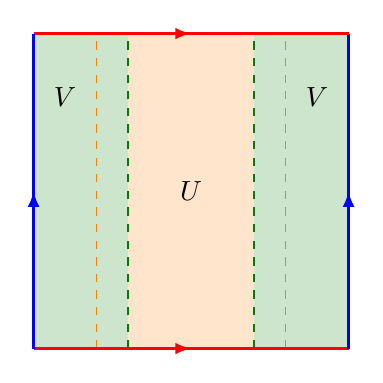
\begin{tikzpicture}[scale=4]
  \fill[orange!20] (0.2,0) rectangle (0.8,1);
  \fill[heavygreen!20] (0,0) rectangle (0.3,1);
  \fill[heavygreen!20] (0.7,0) rectangle (1,1);
  \draw[heavygreen,dashed,line width=0.6pt] (0.3,0)--(0.3,1);
  \draw[heavygreen,dashed,line width=0.6pt] (0.7,0)--(0.7,1);
  \draw[orange,dashed,line width=0.6pt] (0.2,0)--(0.2,1);
  \draw[orange,dashed,line width=0.6pt] (0.8,0)--(0.8,1);
  \draw[red,line width=1pt,midarr] (0,0)--(1,0);
  \draw[blue,line width=1pt,midarr] (1,0)--(1,1);
  \draw[red,line width=1pt,midarr] (0,1)--(1,1);
  \draw[blue,line width=1pt,midarr] (0,0)--(0,1);
  \node at (0.5,0.5) {$U$};
  \node at (0.1,0.8) {$V$};
  \node at (0.9,0.8) {$V$};
\end{tikzpicture}
\end{document}
